\documentclass{IEEEtran}
\usepackage{cite}
\usepackage{amsmath,amssymb,amsfonts}
\usepackage{algorithmicx}
\usepackage{graphicx}
\usepackage{textcomp}
\usepackage{booktabs}
\def\BibTeX{{\rm B\kern-.05em{\sc i\kern-.025em b}\kern-.08em
    T\kern-.1667em\lower.7ex\hbox{E}\kern-.125emX}}
\begin{document}
\title{The Automated Modeling and Optimization of Part DNA Substructures Employing Evolutionary Computation (May 2019)}
\author{Daniel Tauritz, \textit{Senior Member, IEEE}, Jagannathan Sarangapani, Bailey Eversmeyer, National Security Campus}

\maketitle

\begin{abstract}

\end{abstract}

\begin{IEEEkeywords}
Evolutionary computation, Genetic algorithms, Part DNA, Product DNA
\end{IEEEkeywords}

\section{Introduction}
The goal of a Part DNA system is to model and map the flow of goods and products through an area and track the changes as each component moves through the system. The Part DNA system allows the user to identify relationships between components, to conduct analyses on the system: how changes affect the quality or cost of the system \cite{b1}. Our goal in this project is to break down a Part DNA model into key substructures, and optimize the input-output relationship based on quality and cost. We will be using Evolutionary Computation (EC) strategies to help with modeling and optimizing the substructures.

\textbf{[NSC or Jag explanation of part DNA]}

\section{Modeling the Problem}
Given a Part DNA substructure (e.g., a production line), the process of composing products with desired characteristics (e.g., thickness with target tolerance) from source components can be represented as a set of functions that take the input component attributes and their tolerances and produce the output product attributes with their tolerances. Assuming we have perfectly accurate sets of functions, we can simulate using different components to predict the final output component attributes and compare them to the desired results.

\textbf{[NSC or Jag explanation of the real world modeling]}

\section{Computational Challenges}
In order to provide the Decision Maker (DM) with a Pareto-optimal trade-off surface, the Part DNA components to be optimized need to be modeled appropriately for the application of a multi-objective optimizer. An example is trading off cost for output component attribute variation (e.g., cheaper input components may be expected to generally lead to higher variation in the attributes of the output component). A sufficiently high fidelity model is needed in order to accurately test new input component combinations without disrupting the current production lines. The computational challenges are:

\textbf{[Dr. T,  How do I format the contact info in this area?]}

\begin{enumerate}
\item Creating a sufficiently high fidelity model appropriate for multi-objective optimization.
\item Implementing a suitable multi-objective optimizer.
\end{enumerate}

\section{Proposed Solutions}
We propose the following computational approaches to address the computational challenges:
\begin{enumerate}
\item To accurately model the transformation functions which specify how a particular machine in a production line transforms input components to output components and the associated attribute values. For more complex processes, it is likely that the transformation function is nonlinear and not fully specified. This is where we can apply a type of Evolutionary Algorithm (EA), the Genetic Programming (GP) approach, which is used to model mathematical functions and even computer programs. EAs are well suited to exploring search spaces and finding improvements on existing solutions. EAs are stochastic population-based algorithms modeled on biological evolutionary principles of DNA mutation and recombination along with survival of the fittest. With a large enough sample size of input/output pairs, sufficiently accurate functions can be evolved to model the transformations without having to know explicitly how each machine performs each transformation.
\item With the model in hand, we would like to take into account the accuracy of the desired output and the cost of the components provided as inputs, to provide the DM with a diverse Pareto optimal trade-off surface. Multi-Objective EAs (MOEAs) are well suited for exploring spaces that have trade-offs in the possible solutions. For this problem, the MOEA can compare a solution’s accuracy and cost with other solutions and provide a variety of possible solutions that have their own pros and cons. For example, a solution that is very accurate but costs four times more than another solution that is only slightly less accurate. Neither solution is inherently better than the other. So it becomes an issue of how to balance between the two objectives. From our initial work, which utilizes artificial data for the inputs and transformation functions, the MOEA is providing decent Pareto-fronts, which graph the trade-off surface between the objectives.
\end{enumerate}
\begin{figure}[!t]
\centerline{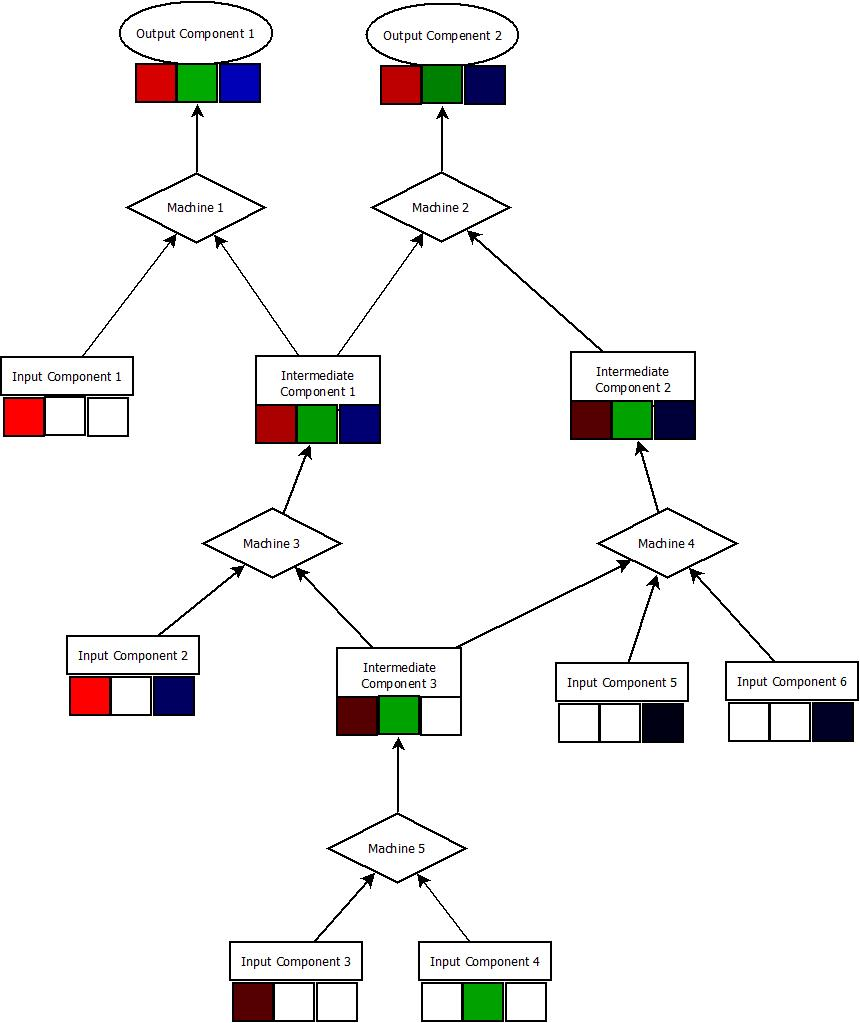
\includegraphics[width=\columnwidth]{Diagram1.jpeg}}
\caption{The above diagram illustrates our modeling approach. Imagine for instance that this example is for creating two types of electrical wire. Red indicates the general durability attribute, green for conductivity, and blue for malleability. The hue indicates a user-defined aspect of a particular component attribute, for instance variation. A darker color designates a lower value, for instance less variation, which is typically associated with higher quality. The different color hues in the diagram demonstrate some of the possible attribute-transformation-interactions, where nonlinear effects between input attributes may translate to the output attributes.}
\label{fig1}
\end{figure}

\section{EC Background}
\subsection{EA Background}
EAs are stochastic, population based local search algorithms based on neo-Darwinian Evolutionary theory \cite{b3}. An EA works by generating solutions and rating them through some fitness fuction. The fitness function is determined by the problem that the EA is trying to solve. For example, trying to maximize the score of a game or the speed at which another algorithm finds a solution. The population members that we use is based on the Survival-of-the-fittest. The more fit a member of the population is, the more likely we chose them to create new population members. The key components to an EA are: the representation, the fitness function, and the operators used to explore the search space.

The representation can be something simple like a bit string, or something more complex like a graph.

The fitness function is how we determine which solutions are better, as the algorithm explores the search space it generally moves towards better solutions. Depending on the layout of the search space and associated fitness, an EA can get stuck in local optima.

The most common operators used to explore the search space are recombination and mutation. Recombination is based on natrual reproduction concepts. By taking multiple population members and combining their DNA in some fashion, we can create a new population member that may have the best pieces of their parents. Mutation is a key factor because it allows us to create new solutions that don't depend on the solutions available from the population. There are many variations to these operators that depend on the representation used, as well as some operators are better suited to specific problems.

\subsection{GP Background}
GP generally represents a solution as a graphical tree-like structure with leaf and internal nodes \cite{b2}. We used a binary tree structure for our models, though a GP solution node can have varying numbers of children depending of the functions allowed. Take, for example, the following equation: 
\begin{equation}
Y = X^2 + sin(X*\pi)
\end{equation}
The GP representation for this equation might look like the tree in Figure 2. To explore the search space of the problem, we use the methods of recombination and mutation to create new solutions. Recombination of two trees is defined as follows:
\begin{itemize}
\item Pick two nodes, one from each tree.
\item Create two children, one copy of each parent.
\item At each chosen node, swap the subtree with the subtree from the other parent.
\end{itemize}
This generates two new trees that are a combination of the two selected parents. The mutation operation is very similar, however, instead of two parents, there is only one. The subtree that is swapped is a new, randomly generated subtree.

\begin{figure}[!t]
\centerline{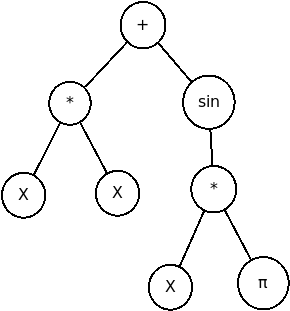
\includegraphics[width=\columnwidth]{functionmodel.png}}
\caption{Binary tree representation of an equation}
\end{figure}

\subsection{MOEA Background}
An MOEA is an EA that uses a fitness value based on multiple objectives \cite{b3}. These objectives are usually in conflict with one another. For example, producing a higher quality item for a higher affordability. Inuitively, as the quality of an item goes up, the affordability will go down. However, something with a high quality and low affordability is not explicitly better than something with low quality and high affordability. This is how an MOEA differs from a regular EA. The MOEA will provide a list of possible solutions that are all equally viable but have trade-offs among each other.

\section{Methodology}
\subsection{Part-DNA Model}
We designed our Part-DNA Model on the principle of taking input components and performing some form of transformation on the input components' attributes and producing an output component. The whole process consisting of a set of transformations based on the list of input and intermediate components leading to a final set of output components. For the purposes of testing, we created two subsets of data for the input component attributes and transformation functions:
\begin{enumerate}
\item Randomly generated values to test GP strategies.
\item Hand made values to test MOEA strategies.
\end{enumerate}
We chose these methods to ensure fitness evaluations would more closely resemble a real-world scenario for the application of the designed methods.


\textbf{[Dr. T,  what kind of 'our model' description do we need? I'm pretty sure we need one, but I keep thinking myself in circles]}
%\subsection{reword}
%In regards to the GP problem,

%As for the MOEA portion, in a real world scenario; the input parameters, as well as intermediate and ouput parameters should be well documented and proper domain and range knowledge


\subsection{GP}
For this problem, we used a binary tree representation to generate our goal functions and to evolve approximations to those functions. We generated leaf nodes from one of the following groups: one of the attributes from any input component, or a constant number, real valued or discrete. Non-leaf nodes used the addition, subtraction, and multiplication operands. For testing the accuracy of the evolved solutions, the fitness was calculated as the sum squared error (SSE) across 64 combinations of input components with an addition of max tree depth to encourage consice representations.
\begin{equation} \label{eq:1}
\begin{split}
fitness=(penaltyfactor)*treedepth \\
+ \sum (expected-result)^{2}
\end{split}
\end{equation}
%Equation \ref{eq:1} shows the fitness function written out.

\begin{table}[!h]
\centering
\caption{GP parameters}
\begin{tabular}{l|l}
\toprule[1.5pt]
Parameter & Value \\\midrule[1pt]
Population Size & 100 \\ 
Number of Offspring & 50 \\
Max Generations & 1000 \\
No Improvement Limit & 35 Generations \\
Recombination Rate & 1.0 \\
Mutation Rate & 0.2 \\
\bottomrule[1.25pt]
\end{tabular}
\end{table}

\subsection{MOEA}
For this problem, we created a model that used three transformation sets (machines) and four types of input components, with each component have four sub-types. The solution is represented as a sub-type selection for each input type. Each solution is rated based on how close it is to the goal component and the total affordability of the input selections. Due to the difficulty in generating input component and output components that fit together through several basic non-linear transformations, we relied on hand made inputs, outputs, and transformations.

\begin{table}[!h]
\centering
\caption{MOEA parameters}
\begin{tabular}{l|l}
\toprule[1.5pt]
Parameter & Value \\\midrule[1pt]
Population Size & 20 \\ 
Number of Offspring & 25 \\
Max Generations & 1000 \\
No Improvement Limit & 10 Generations \\
Recombination Rate & 0.5 \\
Mutation Rate & 0.25 \\
\bottomrule[1.25pt]
\end{tabular}
\end{table}

\section{Results}
\subsection{Sample GP models}
We tested this model on random functions up to depth four and a randomly generated set of 64 input components. Up to depth three, on average half of the transformation functions were modeled accurately with 75 generations. At depth four, average approximations had an SSE value less than 16, or 0.25 units away per input combination.

\subsection{MOEA solutions}
Since our search space was so small, we decided to use smaller population parameters to showcase how an MOEA would move through the Pareto Front in a more realistic scenario. In our sample, there were eighteen total Pareto Optimal combinations. With our small population parameters, the MOEA tended to lose Pareto Optimal solutions because of duplicated individuals and not being able to fit all of the solutions within one population. A second, shorter experiment with population size of 200 and child population size of 250 did converge to the eighteen Pareto Optimal solution within 100 generations on average.

\begin{figure}[!t]
\centerline{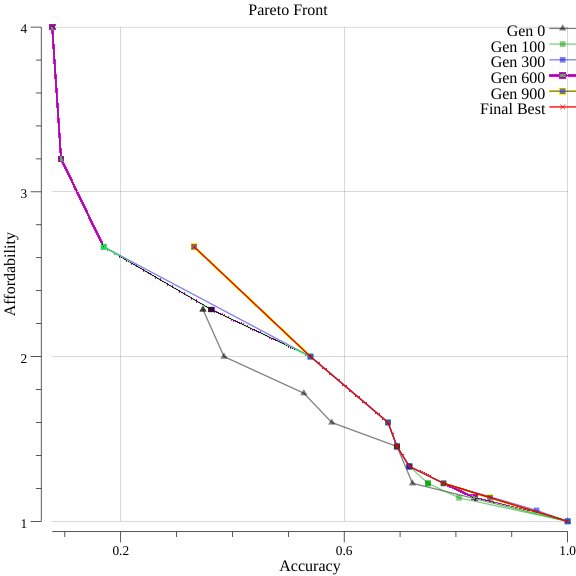
\includegraphics[width=\columnwidth]{points.png}}
\caption{The above diagram shows a Pareto Front graph which plots the set of optimal trade-off points. None of the points shown are entirely better than any other point on the graph. The bottom-right point has the best accuracy, but also has the lowest affordability. The top-left point is the opposite, having the lowest accuracy and highest affordability. Both options have a benfit over the others.}
\end{figure}
\begin{figure}[!t]
\centerline{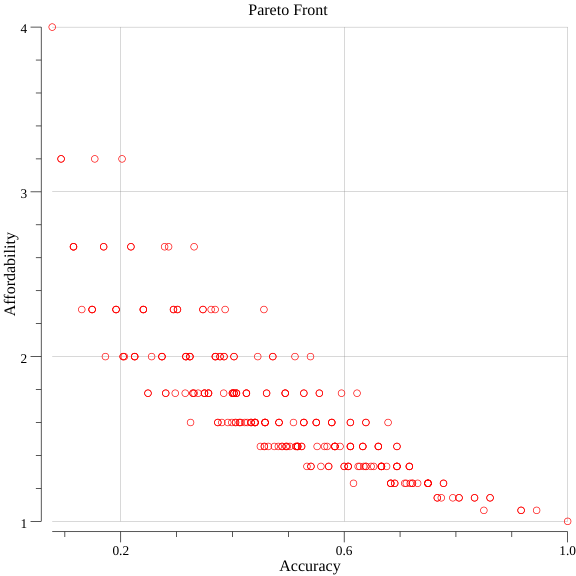
\includegraphics[width=\columnwidth]{all_pareto_points.png}}
\caption{The above diagram shows all the possible Pareto points within our model. There were a total of 256 possible combinations with our hand-made inputs.}
\end{figure}

\section{Future Work}
A natural extension of the proposed work is to simultaneously with the proposed trade-off optimization, also optimize the organization of all the different machines in the plant based on their individual processing times, in order to achieve maximum efficiency. The latter is an instance of the general Job Shop Scheduling problem.

\begin{thebibliography}{00}
\bibitem{b1} https://www.youtube.com/watch?v=cc16ClXGuYQ
\bibitem{b2} John R. Koza.   Hierarchical genetic algorithms operating on populations ofcomputer programs.  In N. S. Sridharan, editor,Proceedings of the Eleventh In-ternational Joint Conference on Artificial Intelligence IJCAI-89, volume 1, pages768–774, Detroit, MI, USA, 20-25 August 1989. Morgan Kaufmann.
\bibitem{b3} A. E. Eiben and J. E. Smith,Introduction to Evolutionary Computing. Second Edition, Springer-Verlag,Berlin Heidelberg, 2015, ISBN 978-3-662-44873-1.
\end{thebibliography}

\end{document}